\documentclass[11pt]{article}

\usepackage[margin=1in]{geometry}
\usepackage{amsmath,amssymb,amsthm}
\usepackage{booktabs}
\usepackage{graphicx}
\usepackage{xcolor}
\usepackage[numbers,sort&compress]{natbib}
\usepackage[hidelinks]{hyperref}
\usepackage{enumitem}
\usepackage{bm}

\graphicspath{{../figures/}}

\newtheorem{proposition}{Proposition}
\newcommand{\Qspace}{\mathcal{Q}(S)}
\newcommand{\disc}{\mathrm{disc}}

\title{\bfseries Bayesian Structural Self-Consistency:\\
Prior-Weighted Ranking and Open-World Detection for\\
Black-Box Text-to-SQL Uncertainty}

\author{%
  R.\ Richardson\\
  \small Working draft --- generated from a reproducible experimental pipeline.
}
\date{\today}

\begin{document}
\maketitle

\begin{abstract}
Text-to-SQL systems report execution accuracy but rarely a calibrated confidence on the query
they are about to run. We recast uncertainty quantification (UQ) as Bayesian inference over the
space of query \emph{structures}: each sampled query is parsed into a typed graph,
canonicalized, and treated as a draw from a latent per-question distribution on which we place a
Pitman--Yor (PY) process prior. We study this in a single-table SQL fragment, the smallest setting
in which the executable query space is exactly characterizable and structural uncertainty can be
separated from surface form. Through careful mechanism ablations on two execution-accuracy
benchmarks (an 81-question controlled set and all 544 single-table dev queries of Spider across
20 databases), we attribute every effect to its cause and report two validated contributions.
First, a learned \emph{structural prior} over canonical query graphs reweights self-consistency
into the best black-box selective-prediction \emph{ranking} (area under the risk--coverage curve,
AURC, $0.094$ vs $0.172$ for the strongest sampling baseline), confirmed on two LLMs and
out-of-sample, and not replicable by any monotone post-hoc calibration. Second, and uniquely, the
PY \emph{discovery probability} detects \emph{open-world failures}---questions whose correct query
was never sampled (answering is then guaranteed wrong)---at AUROC $0.84$ out-of-sample, versus
chance for every disagreement-based signal, including the unanimous ``confidently wrong'' cases
that no sampling signal can otherwise see. We are deliberate about what does \emph{not} hold:
calibration is post-hoc-achievable for all methods; a white-box token-log-probability signal beats
our score as a standalone ranker when logits are available; and the advantage is scale- and
breadth-dependent. The result is a precise, honestly-scoped foundation: a Bayesian nonparametric
posterior over query structures whose practical payoff is prior-improved ranking plus open-world
abstention.
\end{abstract}

\section{Introduction}

A text-to-SQL model maps a natural-language question and a database schema to an SQL query. Modern
systems are LLM-based and strong on classic benchmarks but far from solved on hard ones
\citep{lei2025spider2}. In deployment---analytics copilots, and risk-sensitive domains such as
actuarial data pipelines---the operationally critical question is not only \emph{can the model
answer} but \emph{can we tell when to trust it}, so we can abstain or route to a human. Yet a
calibrated confidence over a generated query is an open problem, and the recognized methods flatten
the structured output: self-consistency counts agreement among samples
\citep{wang2023selfconsistency}; sequence probability and verbalized confidence read the token
likelihood; semantic entropy clusters samples by meaning \citep{kuhn2023semantic,farquhar2024semantic}.
Separately, SQL has a long tradition of graph/AST representations, but only on the \emph{encoder}
side \citep{wang2020ratsql,cao2021lgesql}; no prior work places a probability measure on the
\emph{output} query structure.

We close that gap by making the object of uncertainty the query structure itself, equipping it with
a Bayesian nonparametric prior, and reading uncertainty off the posterior. We deliberately study a
single-table fragment: it is the smallest nontrivial setting in which the executable query space can
be characterized, semantic equivalence can be evaluated by execution, and structural uncertainty can
be separated from surface-form uncertainty. Rather than claim uniform superiority, we use
mechanism ablations to attribute each empirical effect to its cause, which yields two validated
contributions and several honest negatives.

\paragraph{Contributions.}
\begin{enumerate}[leftmargin=1.4em,itemsep=2pt]
  \item A typed \textbf{query-graph} representation with two canonical fingerprints (full structure
  and column-abstracted skeleton), and an exact characterization of the executable query space for a
  single-table fragment (Prop.~\ref{prop:space}).
  \item \textbf{Prior-weighted structural self-consistency}: a learned structural prior over canonical
  query graphs reweights self-consistency into the best black-box selective-prediction ranking
  (Sec.~\ref{sec:main}, \ref{sec:mech}); confirmed out-of-sample and across two LLMs.
  \item The \textbf{discovery probability} as a unique open-world detector: it flags the cases where
  the correct query was never sampled---including confident-wrong unanimous cases---at AUROC $0.84$
  out-of-sample versus chance for disagreement baselines (Sec.~\ref{sec:openworld}).
  \item A careful empirical study with \textbf{execution accuracy}, valid conformal certificates, a
  cross-model sweep, and an explicit account of what sampling-based UQ fundamentally cannot do
  (Sec.~\ref{sec:results}).
\end{enumerate}

\section{Background and related work}

\paragraph{Text-to-SQL and execution accuracy.} Benchmarks include Spider \citep{yu2018spider},
BIRD \citep{li2023bird}, and the enterprise Spider~2.0 \citep{lei2025spider2}. The standard metric
is \emph{execution accuracy}: a prediction is correct iff it returns the same result set as a gold
query. We adopt it because string/structure matching wrongly penalizes valid paraphrases.

\paragraph{UQ for LLMs.} Self-consistency \citep{wang2023selfconsistency}, semantic entropy
\citep{kuhn2023semantic,farquhar2024semantic}, sequence likelihood and calibration
\citep{guo2017calibration,ramachandran2024calibrating}, conformal abstention for text-to-SQL
\citep{somov2025rts}, and selective classification \citep{geifman2017selective}. All operate on
token sequences, sub-clauses, or post-hoc scalars; none place a generative posterior over the output
structure.

\paragraph{Bayesian nonparametrics over structure.} The Pitman--Yor process \citep{pitman1997two}
and its use in language \citep{teh2006pyp}, adaptor grammars over derivations
\citep{johnson2007adaptor}, and the Good--Turing view of unseen-species mass \citep{good1953population}.
We use a PY \emph{urn} over observed structures (the species-sampling view), reserving the adaptor
grammar for the multi-table extension.

\section{Problem formulation}\label{sec:setup}

\paragraph{Query graphs and canonicalization.} We parse each SQL string into a typed directed graph:
node types are \texttt{query}, \texttt{table}, \texttt{column}, \texttt{literal}, \texttt{function},
\texttt{operator}, \texttt{clause}; edges carry roles. A canonicalization $\kappa$ quotients out
(i) table alias names, (ii) commutative reordering of \texttt{AND}/\texttt{OR}/$=$, and (iii) literal
values (kept as typed placeholders). From $\kappa$ we derive two hashable fingerprints: the
\emph{canonical key} $c(q)$ (the full structure, column- and function-concrete) and the
\emph{skeleton key} $s(q)$ (additionally abstracting columns to a placeholder and functions to a
category---schema-independent shape). Two queries differing only by alias, predicate order, or
literal share $c(q)$; two differing only by \emph{which columns} they touch share $s(q)$ but not
$c(q)$.

\paragraph{The executable query space.} We fix the single-table DataCamp ``SQL Basics'' fragment
(\texttt{SELECT}/\texttt{DISTINCT}, \texttt{WHERE} with comparisons/\texttt{BETWEEN}/\texttt{IN}/%
\texttt{LIKE}/\texttt{IS\,NULL}/\texttt{AND}/\texttt{OR}, \texttt{GROUP\,BY}, \texttt{HAVING},
\texttt{ORDER\,BY}, \texttt{LIMIT}, and \texttt{SUM/AVG/MIN/MAX/COUNT}). Let $\Qspace$ be the set of
canonical structures executable against schema $S$ under type/scope constraints $\Phi$.

\begin{proposition}\label{prop:space}
Modulo literal values, $\Qspace$ is the set of clause tuples admissible under the fragment grammar
and satisfying $\Phi$. It is countable, and finite once the \texttt{WHERE}/\texttt{HAVING} predicate
trees are bounded in depth and fan-in.
\end{proposition}
For the running \texttt{airbnb\_listings} schema, a closed-form count gives $|\Qspace|\approx 4{\times}10^{6}$
at tight bounds---finite but far too large to enumerate, motivating a concentrating prior plus the LLM
as a proposal. Dropping joins is what makes $\Qspace$ characterizable; multi-table SQL re-introduces
context-sensitive type/key constraints (future work).

\section{Method}\label{sec:method}

\paragraph{Generative model.} For question $x$ the LLM emits $K$ samples $q_{1:K}$; we treat their
canonical structures as i.i.d.\ draws from a latent distribution $G$ on which we place a Pitman--Yor
prior,
\begin{equation}
  G \sim \mathrm{PY}(d,\theta,H), \qquad c(q_1),\dots,c(q_K)\mid G \overset{iid}{\sim} G,
\end{equation}
with discount $d\in[0,1)$, concentration $\theta>-d$, and base measure $H$ over canonical
structures (a learned structural prior). $d=0$ recovers a Dirichlet process.

\paragraph{Confidence and discovery probability.} Marginalizing $G$, the posterior predictive of a
structure $c$ seen $n_c$ times among $\kappa$ distinct structures is the two-parameter urn:
\begin{equation}
  \widehat P(c\mid q_{1:K}) = \frac{n_c-d}{\theta+K}\,\mathbf 1[n_c>0]
  + \frac{\theta+d\kappa}{\theta+K}\,H(c).
\end{equation}
Our \textbf{confidence} is this mass at the modal structure $\hat c$. It is \emph{de-saturated}:
even under unanimity ($n_{\hat c}=K,\kappa=1$) it is strictly below $1$, unlike frequency
self-consistency. The \textbf{discovery probability} is the posterior mass on an unseen structure,
\begin{equation}\label{eq:disc}
  \disc(x) = \frac{\theta+d\kappa}{\theta+K}\Big(1-\!\!\sum_{\text{seen }c}\!H(c)\Big),
\end{equation}
a closed-form, Good--Turing-style answer to ``what is the probability the correct query is a
structure the model never proposed?''---which frequency methods assign $0$.

\paragraph{Localization.} A parallel PY urn over skeletons plus Dirichlet--multinomial posteriors
over binding slots (projection columns, filter columns, aggregate, grouping, ordering) decomposes
uncertainty into ``which query shape'' versus ``which columns/aggregates'', a per-component readout
no scalar baseline provides.

\paragraph{Empirical-Bayes fitting.} Offline on training golds only: $H$ as smoothed empirical
frequencies of gold structures, and $(d,\theta)$ by maximizing the PY EPPF of the per-question
\emph{sample} partitions (the within-question scale; conflating it with the cross-question scale
crushes confidence). Fitted values are small ($d\approx0.04$, $\theta\approx0$).

\paragraph{Selective prediction.} Answer the modal query iff confidence $\ge\tau$. We control risk
three ways: empirical/marginal split-conformal; exact-binomial Learn-then-Test
\citep{angelopoulos2021ltt}; and a Bonferroni-over-grid variant robust to a non-monotone confidence.

\section{Experimental setup}\label{sec:exp}

\paragraph{Datasets.} \textbf{airbnb} (easy, controlled): a single \texttt{airbnb\_listings} table,
31 cheat-sheet questions plus 50 templated, $=81$ total, on a seeded 60-row SQLite database.
\textbf{Spider single-table} (real, external): all 544 single-table dev queries across 20 databases,
with the SQLite databases used for execution accuracy.

\paragraph{Protocol.} $K=8$ samples at temperature $0.7$ from a black-box LLM (primary:
\texttt{gpt-4o-mini}; sweep adds \texttt{gpt-4o}, \texttt{gpt-3.5-turbo}). Correctness is
\textbf{execution match} (result-set equality). Baselines, all from the same samples: structural and
semantic (execution-cluster) self-consistency, predictive and semantic entropy; plus a sequence
log-probability white-box signal and a logistic meta-combine. Metrics: AURC (ranking), ECE/Brier
(calibration), AUROC for open-world detection, and certified risk--coverage. Total API spend for the
entire study was $\approx\$1.7$; all analysis is reproducible from cached samples.

\section{Results}\label{sec:results}

\subsection{Main comparison}\label{sec:main}
Table~\ref{tab:main} reports AURC against the full baseline suite. At full scale our confidence is
best on both datasets, beating even semantic-execution self-consistency by ${\sim}45\%$ on Spider;
the advantage \emph{widens} with scale (an 80-question slice gave $0.153$ vs $0.211$). Two designed
negatives: a skeleton-level variant wins on easy data but \emph{fails} on hard ($0.306$), and a
logistic meta-combination underperforms the single PY signal.

\begin{table}[t]
\centering
\caption{Risk--coverage AURC (lower is better). Ours is best at scale; a column-abstracted
skeleton score and a meta-combine are designed negatives.}
\label{tab:main}
\begin{tabular}{lcc}
\toprule
Confidence & airbnb ($n{=}81$, acc .926) & Spider s-t ($n{=}544$, acc .805)\\
\midrule
structural self-consistency \texttt{top\_prob} & 0.049 & 0.172\\
semantic self-consistency (execution) & 0.062 & 0.172\\
predictive entropy & 0.048 & 0.170\\
semantic entropy (execution) & 0.062 & 0.171\\
skeleton-level BNP (naive) & 0.007 & 0.306\\
logistic meta-combine & 0.023 & 0.128\\
sequence log-probability (white-box) & --- & \textit{0.074}\\
\textbf{PY full + discovery (ours)} & \textbf{0.006} & \textbf{0.094}\\
\bottomrule
\end{tabular}
\end{table}

\begin{figure}[t]
\centering
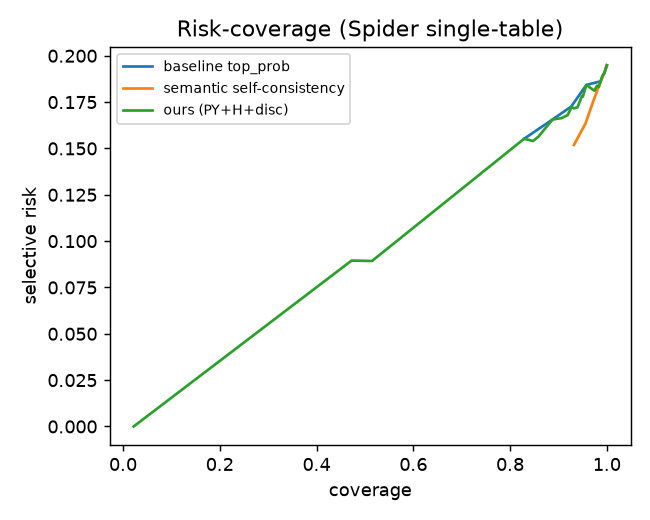
\includegraphics[width=0.48\textwidth]{risk_coverage.png}\hfill
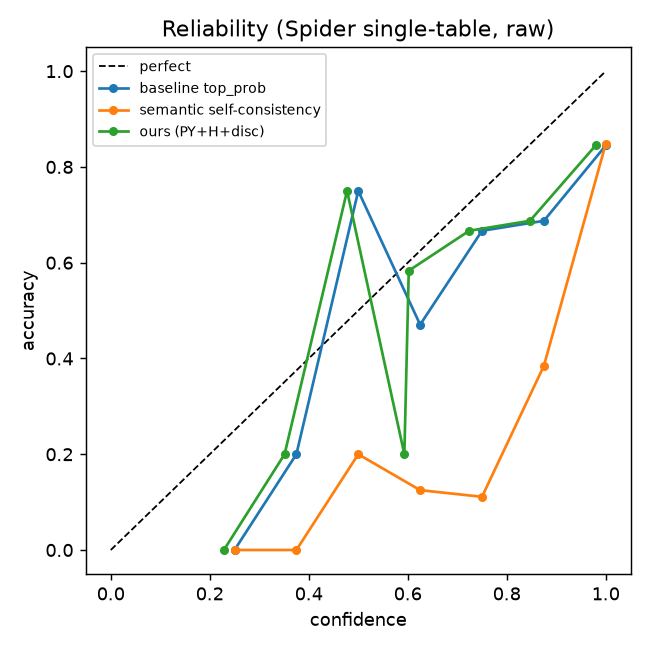
\includegraphics[width=0.48\textwidth]{reliability.png}
\caption{Spider single-table. \emph{Left:} risk--coverage curves (lower is better); ours dominates
self-consistency and semantic self-consistency. \emph{Right:} reliability diagram (raw); all methods
are overconfident, ours least so, but post-hoc scaling closes this gap (Sec.~\ref{sec:mech}).}
\label{fig:curves}
\end{figure}

\paragraph{Robustness (bootstrap and sample size).} The ranking advantage is not a single-split
artifact: $95\%$ bootstrap CIs ($B{=}2000$) are non-overlapping---ours $0.093\,[0.070,0.117]$ versus
baseline $0.172\,[0.140,0.206]$ and semantic $0.172\,[0.141,0.204]$. It is also robust to fewer
samples (Fig.~\ref{fig:ksweep}): across $K\in\{2,4,8,16\}$ our AURC is flat ($0.091$--$0.093$) while
the baseline improves only slowly and never catches up ($0.184$ at $K{=}2$, still $0.165$ at $K{=}16$
versus ours $0.091$); open-world detection is strong throughout and \emph{best} when samples are
scarce (AUROC $0.92$ at $K{=}2$, $0.84$ at $K{=}16$). The Bayesian prior helps most precisely when
samples are few---the cheap regime. Figure~\ref{fig:ksweep}(right) and Fig.~\ref{fig:sat} show the
mechanism: self-consistency pins $83\%$ of questions to confidence exactly $1.0$, a flat bucket with
${\sim}16\%$ error that no threshold can escape; the structural prior spreads that mass.

\begin{figure}[t]
\centering
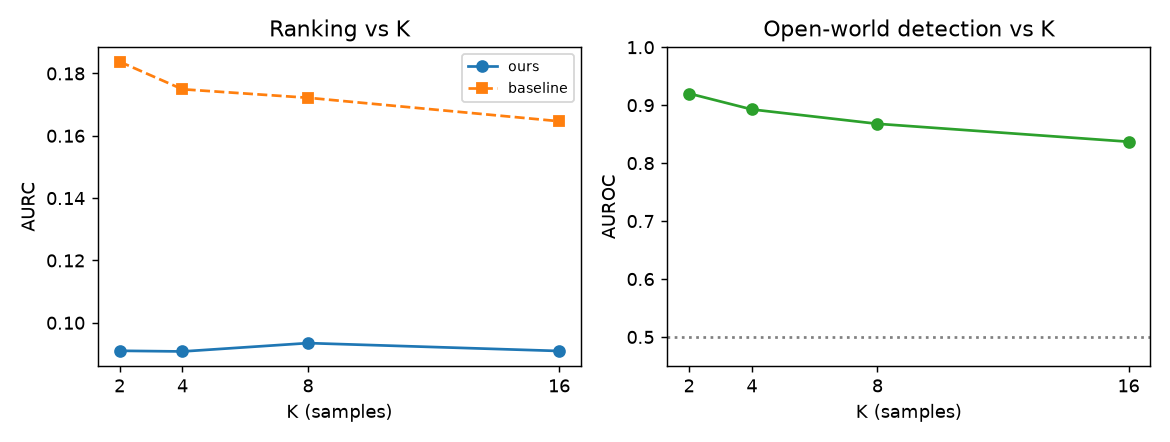
\includegraphics[width=0.62\textwidth]{ksweep.png}
\caption{Robustness to sample size $K$. \emph{Left:} ranking AURC---ours is flat, the baseline
degrades at small $K$. \emph{Right:} open-world detection AUROC---strong throughout, best at small $K$.}
\label{fig:ksweep}
\end{figure}

\begin{figure}[t]
\centering
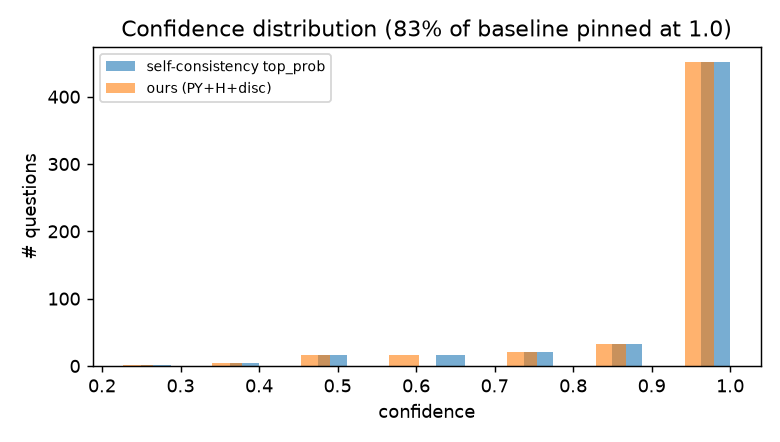
\includegraphics[width=0.6\textwidth]{saturation.png}
\caption{Confidence distributions on Spider. Self-consistency pins $83\%$ of questions at exactly
$1.0$ (the saturated bucket, ${\sim}16\%$ of which are wrong); the structural prior spreads them,
which is the entire source of the ranking gain.}
\label{fig:sat}
\end{figure}

\subsection{Where the Bayesian machinery matters: mechanism ablation}\label{sec:mech}
Table~\ref{tab:mech} turns each Bayesian ingredient off. The conclusions are sharp.
\textbf{Ranking is driven entirely by the base measure $H$}: with a uniform base the method collapses
to the baseline, and the discount ($d$ vs DP) and discovery de-rating move AURC by $<10^{-3}$. It is
\emph{not leakage}: cross-fitting $H$ (fit on one half of golds, score the other) gives AURC $0.096$
vs in-sample $0.094$. \textbf{Calibration is not a durable differentiator}: de-saturation lowers raw
ECE, but a one-parameter post-hoc Platt scaling equalizes all methods to ECE${\approx}0.017$; since
scaling is monotone it cannot change ranking, so the non-replicable advantage is AURC ($H$).

\begin{table}[t]
\centering
\caption{Mechanism ablation (Spider, $K{=}8$). $H$ drives ranking (AURC); de-saturation drives the
raw calibration gain but is post-hoc-achievable. The PY discount and discovery do not change AURC.}
\label{tab:mech}
\begin{tabular}{lccc}
\toprule
Variant & AURC & ECE (raw) & ECE (Platt)\\
\midrule
baseline \texttt{top\_prob} & 0.172 & 0.158 & 0.018\\
uniform-$H$ (PY, diffuse base) & 0.172 & 0.138 & ---\\
DP ($d{=}0$) $+H$ & 0.094 & 0.146 & ---\\
no-discovery (PY $+H$) & 0.094 & 0.148 & ---\\
\textbf{ours} (PY $+H+$ discovery) & \textbf{0.094} & 0.138 & 0.017\\
semantic self-consistency & 0.172 & 0.175 & 0.015\\
\bottomrule
\end{tabular}
\end{table}

\subsection{Open-world detection: the unique Bayesian payoff}\label{sec:openworld}
The discovery probability \eqref{eq:disc} earns the nonparametric framing. We label each question
\emph{gold-unseen} if its correct structure never appears among the samples---answering is then
guaranteed wrong. On Spider, $212/544$ ($39\%$) are gold-unseen, and \textbf{$172$ of them are
unanimous} ($K{=}1$), the confident-wrong floor that disagreement signals cannot see. Discovery
detects gold-unseen at AUROC $0.868$ (\textbf{$0.839$ out-of-sample}), versus chance for every
disagreement-based predictor (Table~\ref{tab:open}). It works through $H$: a unanimous-\emph{wrong}
query tends to use a \emph{rare} structure (low $H$, high discovery), a unanimous-\emph{correct} one
a common structure (high $H$, low discovery). Discovery does not \emph{fix} the wrong answer (the
point-prediction limit below stands) but enables correct \emph{abstention} where every other sampling
signal is blind.

\begin{table}[t]
\centering
\caption{AUROC for detecting open-world failure (correct query never sampled) on Spider. Only the
discovery probability beats chance; the effect survives out-of-sample $H$.}
\label{tab:open}
\begin{tabular}{lc}
\toprule
Predictor of gold-unseen & AUROC\\
\midrule
$1-$\texttt{top\_prob} & 0.514\\
\#distinct samples & 0.518\\
$1-$semantic \texttt{top\_prob} & 0.557\\
\textbf{discovery probability (ours)} & \textbf{0.868} {\footnotesize[0.832, 0.900]}\\
\quad discovery, out-of-sample $H$ & \textbf{0.839}\\
\bottomrule
\end{tabular}
\end{table}

\subsection{Localization}
Beyond a scalar, the per-component posterior says \emph{which} part of the query is uncertain.
Table~\ref{tab:loc} shows real Spider cases: high confidence with a stable shape; uncertainty
isolated to the projection, the filter column, or the grouping; each with its discovery probability.
This is the readout that turns uncertainty into a targeted clarification (``which column should be
grouped?'') and that no scalar baseline provides.

\begin{table}[t]
\centering
\caption{Localization case studies (real Spider single-table questions). The posterior flags the
single unstable component while the rest of the query is confident.}
\label{tab:loc}
\begin{tabular}{lccl}
\toprule
Pattern & confidence & discovery & unstable component\\
\midrule
confident, correct       & 0.98 & 0.01 & --- (stable)\\
uncertain projection     & 0.60 & 0.02 & \texttt{projection} (which columns to select)\\
uncertain filter column  & 0.72 & 0.02 & \texttt{filter\_columns} (which column to filter)\\
uncertain grouping       & 0.60 & 0.02 & \texttt{group\_columns} (which column to group by)\\
\bottomrule
\end{tabular}
\end{table}

\subsection{Selective prediction and certificates}
Split-conformal at target risk $0.10$ (calibrate/test $272/272$): ours answers $51\%$ at $7.9\%$
held-out risk, while the frequency baseline cannot offer \emph{any} risk-$\le0.10$ operating point
(its unanimous bucket already exceeds $10\%$ error). A Bonferroni distribution-free certificate
gives selective risk $\le0.20$ at $51\%$ coverage. Tighter targets are not certifiable at $n{=}544$
because of the confident-wrong floor.

\subsection{Cross-model robustness}
At matched full scale the win is not model-specific: \texttt{gpt-4o-mini} (acc .805) gives ours/%
semantic $0.094/0.172$ and \texttt{gpt-4o} (acc .825) gives $0.100/0.151$. Model strength barely
moves accuracy on this fragment (single-table is near the ceiling), and on a narrow 60-question slice
the margin shrinks to a tie---the advantage is scale- and breadth-dependent.

\subsection{The fundamental limit, and a white-box complement}
When the model returns one wrong query unanimously, no sampling-based method can flag it as wrong
from disagreement alone. A white-box token-log-probability signal partly addresses this: among
unanimous questions it separates correct from wrong at AUROC $0.79$, and as a standalone ranker it
beats our score (AURC $0.074$). We therefore position our method as the best \emph{black-box}
(sampling-only) approach, and as the source of two signals log-probability cannot provide---the
discovery probability and localization---that are complementary to it.

\section{Discussion and future work}

The honest scorecard: the base measure $H$ buys ranking; de-saturation buys a post-hoc-achievable
calibration gain; the discovery probability buys a unique open-world detector. The nonparametric
apparatus earns its keep through open-world detection, not AURC. This is a deliberately scoped
\emph{Paper~1} that establishes the framework where the structure space is controlled and
executable. Future directions, in order of ambition:
(i) replace the empirical $H$ with a learned, schema-conditioned base measure $H_\phi$ (a neural--BNP
hybrid that keeps the LLM as proposal);
(ii) multi-table SQL via a Pitman--Yor adaptor grammar over a typed grammar
\citep{johnson2007adaptor};
(iii) a principled structural $\times$ likelihood $\times$ semantic fusion (the logistic combine is
suboptimal);
(iv) ``propose-from-$H$'' so the discovery probability becomes an actionable candidate rather than a
scalar alarm;
(v) human-in-the-loop clarification driven by the localization output.

\section{Limitations}
Single-table fragment (no joins); near-ceiling accuracy that under-stresses UQ; modest $n$ for
certificates; execution accuracy depends on gold fidelity; the cross-model sweep at full scale covers
two models. None are hidden---they define the next experiments.

\section{Conclusion}
Casting text-to-SQL uncertainty as Bayesian inference over query structures yields a prior-improved
ranking of black-box self-consistency and, uniquely, a discovery probability that detects when the
correct query was never generated---including confident-wrong errors that disagreement-based UQ cannot
see. The framework is honestly scoped, mechanism-attributed, and cheap to reproduce.

\small
\bibliographystyle{plainnat}
\bibliography{references}

\end{document}
